\documentclass[tikz,border=10pt]{standalone}
\begin{document}

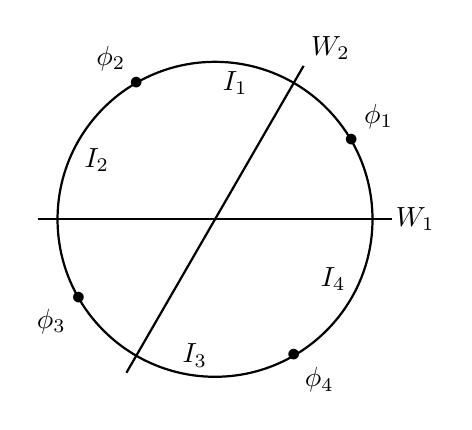
\begin{tikzpicture}
  % Draw the circle
  \draw[thick] (0, 0) circle (2cm);

  % Define the points
  \foreach \angle/\label in {30/\phi_1, 120/\phi_2, 210/\phi_3, 300/\phi_4} {
    % Calculate the coordinates
    \coordinate (p) at ({2*cos(\angle)},{2*sin(\angle)});
    \node at (p) [label={[label distance=-.2cm]\angle:$\label$}] {$\bullet$};
  }

  \draw[thick] (-2.25,0) -- (2.25,0); 
  \draw[thick] ({-2.25*cos(60)}, {-2.25 * sin(60)}) -- ({2.25*cos(60)}, {2.25 * sin(60)});
  \node at (2.25,0) [label={[label distance=-.2cm ]0:$W_1$}] {}; 
  \node at ({2.25*cos(60)}, {2.25 * sin(60)}) [label={[label distance=-.2cm]60:$W_2$}] {}; 

  \foreach \angle/\label in {75/I_1, 150/I_2, 255/I_3, 330/I_4} {
    \coordinate (p) at ({2*cos(\angle)},{2*sin(\angle)});
    \node at (p) [label={[label distance=-.2cm]{\angle+180}:$\label$}] {};
  }  
\end{tikzpicture}
\end{document}
